\chapter{Diseño e Implementación} % Main chapter title

\label{Chapter3} % Change X to a consecutive number; for referencing this chapter elsewhere, use \ref{ChapterX}
\definecolor{mygreen}{rgb}{0,0.6,0}
\definecolor{mygray}{rgb}{0.5,0.5,0.5}
\definecolor{mymauve}{rgb}{0.58,0,0.82}

\lstset{ %
  backgroundcolor=\color{white},   % choose the background color; you must add \usepackage{color} or \usepackage{xcolor}
  basicstyle=\footnotesize,        % the size of the fonts that are used for the code
  breakatwhitespace=false,         % sets if automatic breaks should only happen at whitespace
  breaklines=true,                 % sets automatic line breaking
  captionpos=b,                    % sets the caption-position to bottom
  commentstyle=\color{mygreen},    % comment style
  deletekeywords={...},            % if you want to delete keywords from the given language
  %escapeinside={\%*}{*)},          % if you want to add LaTeX within your code
  %extendedchars=true,              % lets you use non-ASCII characters; for 8-bits encodings only, does not work with UTF-8
  %frame=single,	                   % adds a frame around the code
  keepspaces=true,                 % keeps spaces in text, useful for keeping indentation of code (possibly needs columns=flexible)
  keywordstyle=\color{blue},       % keyword style
  language=[ANSI]C,					% the language of the code
  %otherkeywords={*,...},           % if you want to add more keywords to the set
  numbers=left,                    % where to put the line-numbers; possible values are (none, left, right)
  numbersep=5pt,                   % how far the line-numbers are from the code
  numberstyle=\tiny\color{mygray}, % the style that is used for the line-numbers
  rulecolor=\color{black},         % if not set, the frame-color may be changed on line-breaks within not-black text (e.g. comments (green here))
  showspaces=false,                % show spaces everywhere adding particular underscores; it overrides 'showstringspaces'
  showstringspaces=false,          % underline spaces within strings only
  showtabs=false,                  % show tabs within strings adding particular underscores
  stepnumber=1,                    % the step between two line-numbers. If it's 1, each line will be numbered
  stringstyle=\color{mymauve},     % string literal style
  tabsize=2,	                   % sets default tabsize to 2 spaces
  title=\lstname,                   % show the filename of files included with \lstinputlisting; also try caption instead of title
  morecomment=[s]{/*}{*/}%
}

En este capítulo se presenta la arquitectura del \textit{firmware} y el patrón de diseño usado para los módulos del sistema. Asimismo, se detallan aspectos funcionales de cada módulo y se fundamentan las elecciones de los distintos componentes de hardware utilizados.

El código fuente asociado puede consultarse en la siguiente URL:
\url{https://github.com/alesuarez/soniforo}

%----------------------------------------------------------------------------------------
%	SECTION 1
%----------------------------------------------------------------------------------------
\section{Arquitectura}
A este proyecto se le dió el nombre de Soniforo, de la conjunción da las palabras Sonido y semáforo.

Se optó por un modelo de capas jerárquico para organizar el código en los distintos niveles de abstracción.

En la figura \ref{fig:arquitecturaFirmwareGeneralSistema} se puede observar como se planteó este trabajo. 
 \begin{figure}[h]
	\centering
	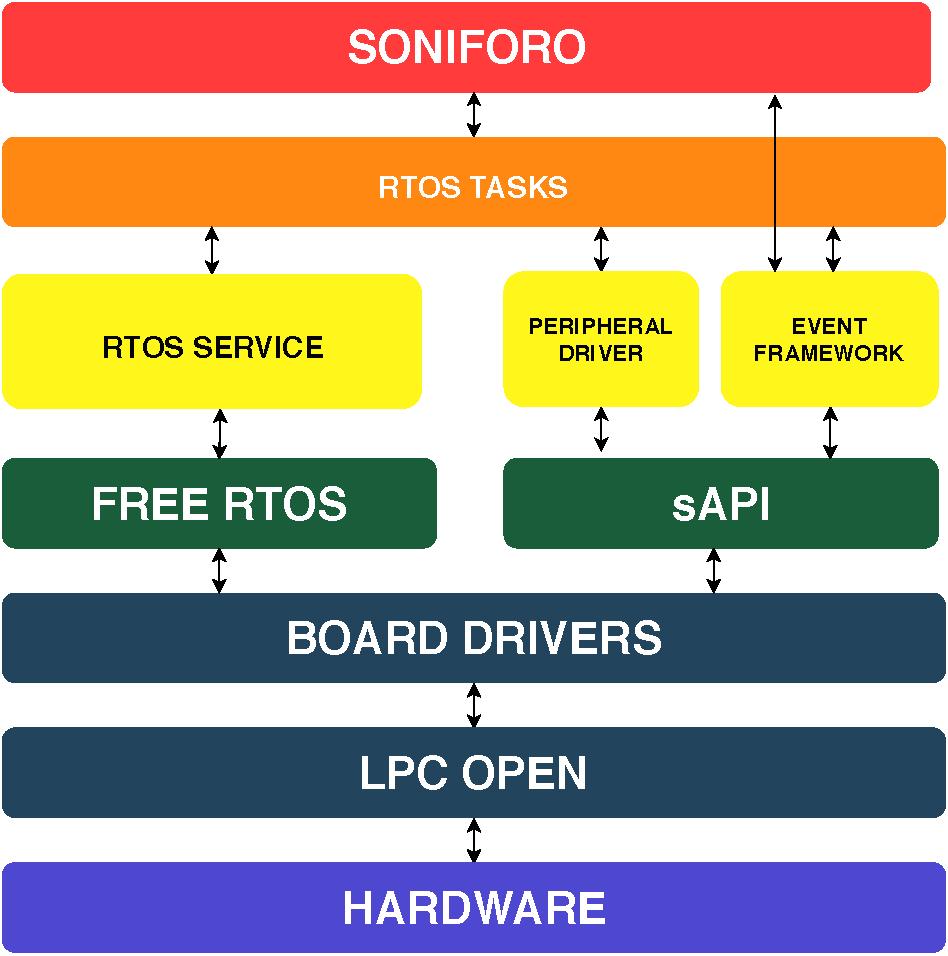
\includegraphics[scale=.6]{./Figures/arquitecturaGeneralSistema.pdf}
	\caption{Estructura de capas para el \textit{firmware}.}
	\label{fig:arquitecturaFirmwareGeneralSistema}
\end{figure}

En cuanto a los niveles de abstraccion, la primera capa consituye el hardware de la plataforma EDU-CIAA. La segunda capa, \textit{Hardware Abstracion Layer} (HAL), permite desacoplar las capas superiores del hardware. Aquí se encuentran los
drivers del fabricante del microcontrolador, en el bloque funcional LPC Open. La capa Hardware Independent Layer (HIL) incluye los módulos del RTOS (no está asociada a ningún hardware en particular) y sAPI que permite el manejo de los perifericos de la placa con mayor facilidad.
Sobre esta base se observa una capa orientada a servicio que nos permiten procesar la información del sistema, estas son: 
\begin{itemize}
\item Rtos service: Se encarga de la creación de tareas, temporizadores, semaforos binarios.
\item Peripheral driver: Se encarga de la configuración de los perifericos, como ser las interrupciones.
\item Envent framework: esta capa se encarga de la definición y creación de todos los eventos del sistema.
\end{itemize}

Sobre estas capas se ubican todas las tareas que corren y son propias del sistema, a esta se la llama Rtos task. Finalmente, la última capa contiene la aplicación Soniforo.



